\documentclass[conference,10pt]{IEEEtran}
%\documentclass[conference,draft,onecolumn]{IEEEtran}
% useful packages, copy and paste from diff sources

\usepackage[english]{babel}
\usepackage[T1]{fontenc}
\usepackage{cite,url,color} % Citation numbers being automatically sorted and properly "compressed/ranged".
\usepackage{graphics,amsfonts}
\usepackage{epstopdf}
\usepackage[pdftex]{graphicx}
\usepackage[cmex10]{amsmath}
% Also, note that the amsmath package sets \interdisplaylinepenalty to 10000
% thus preventing page breaks from occurring within multiline equations. Use:
\interdisplaylinepenalty=2500
% after loading amsmath to restore such page breaks as IEEEtran.cls normally does.
\usepackage[utf8]{inputenc}
% Useful for displaying quotations
%\usepackage{csquotes}
% Compact lists
%\let\labelindent\relax
\usepackage{enumitem}
\usepackage{fancyhdr}
\fancyfoot[C]{\thepage}
%tikz figures
\usepackage{tikz}
\usetikzlibrary{automata,positioning,chains,shapes,arrows}
\usepackage{pgfplots}
\usetikzlibrary{plotmarks}
\newlength\fheight
\newlength\fwidth
\pgfplotsset{compat=newest}
\pgfplotsset{plot coordinates/math parser=false}

\usepackage{array}
% http://www.ctan.org/tex-archive/macros/latex/required/tools/
%\usepackage{mdwmath}
%\usepackage{mdwtab}
%mdwtab.sty	-- A complete ground-up rewrite of LaTeX's `tabular' and  `array' environments.  Has lots of advantages over
%		   the standard version, and over the version in `array.sty'.
% *** SUBFIGURE PACKAGES ***
%\usepackage[tight,footnotesize]{subfigure}
\usepackage{subfig}

\usepackage[top=1.5cm, bottom=2cm, right=1.6cm,left=1.6cm]{geometry}
\usepackage{indentfirst}

\usepackage{times}
% make sections titles smaller to save space
%\usepackage{sectsty}
%\sectionfont{\large}
% enable the use of 'compactitem', a smaller 'itemize'
%\usepackage{paralist}

% MP
% to split equations using dmath env
\usepackage{breqn}
% nice rules in tables
\usepackage{booktabs}

%\setlength\parindent{0pt}
\linespread{1}

% MC
\newcommand{\MC}[1]{\textit{\color{red}MC says: #1}}
\newcommand{\AZ}[1]{\textit{\color{blue}AZ says: #1}}
\newcommand{\MP}[1]{\textit{\color{green}MP says: #1}}

\usepackage{placeins}

\mainmatter
%%%%%%%%%%%%%%%%%%%%%%%%%%%%%%%%%%%%%%%%%%
\begin{document}
%%%%%%%%%%%%%%%%%%%%%%%%%%%%%%%%%%%%%%%%%%
\title{Quality of Service with Software Defined Network.}

\author{\IEEEauthorblockN{Andrea Pittaro, Matteo Maso }
\IEEEauthorblockA{Department of Information Engineering, University of Padova -- Via Gradenigo, 6/b, 35131 Padova, Italy\\Email: {\tt\{pittaroa,masomatt\}@dei.unipd.it}
}}

\maketitle

\begin{abstract}
Quality of Service(QoS) in existing network architectures is an ongoing problem.
A lot of researcher and industries try to solve this problem with many solution but a lot of them are too
expensive other failed or are not implemented.
Software Defined Networking(SDN) paradigm has emerged in response to limitations of traditional networking architectures.
The main advantages of SDN are centralized global network view. This particular features have got attention of researchers to improve QoS.
In questo report mostreremo quali sono stati i principali risutati raggiunti e i problemi incontrati nella realizzazione di
un applicativo SDN in grado di supportare un servizio di tipo QoS.
Lo standard OpenFlow e il controller python POX largamente diffuso sono stati gli strumenti che hanno reso possibile la
realizzazione di quest'esperienza pur mostrando i limiti dovuti all'utilizzo di una tecnologia nuova e in fase di ricerca.
%translate
\end{abstract}

\section{Introduction}\label{sec:intro}
Software-defined networking (SDN) is way to manage networks that separates the control plane from the forwarding plane.
SDN offers a centralized view of the network, giving an SDN Controller the ability to act as the “brains” of the network.
The SDN Controller relays information to switches and routers via southbound APIs, and to the applications with northbound APIs.
One of the most well-known protocols used by SDN Controllers is OpenFlow, however, it isn’t the only SDN standard, but it is widely accepted.
Centralized, programmable SDN environments can easily adjust to the rapidly changing needs of businesses. SDN can lower costs and limit
wasteful provisioning, as well as provide flexibility and innovation for networks.
\#TODO da completare
  \subsection{OpenFlow}
  During 2006 thanks to M. Casado was developed Ethane a new network architecture on this conncept during 2011 was bord the Open Network Foundatin.
  This is a no profit association that would innovate SDN and standardize OpenFlow protocol whit relatives tecnology \cite{ONF}.
  The first version of OpenFlow is 1.0.0 release on 2009 but the last standardized version is v1.5.1 approved on march 2015 \cite{ONF_report}.
  \#TODO da sistemare
\begin{figure}[!h]
 \centering
 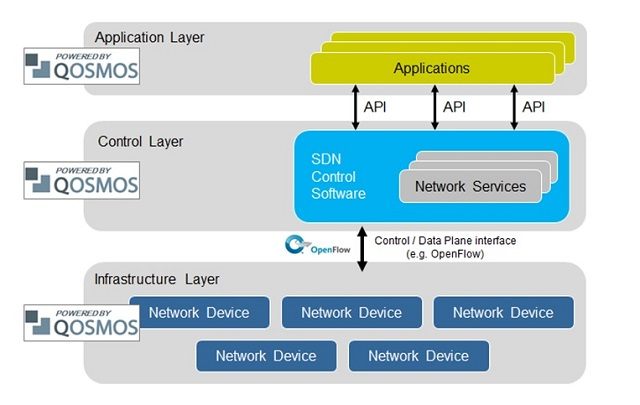
\includegraphics[scale=0.58]{images/of.jpg}
 \caption{\emph{OpenFlow}}
 \label{fig:topo}
\end{figure}
  \\
  \textbf{Openflow 1.0 messages}
Openflow defines a number of messages between a controller and a switch. Now there will be presented some messages we exploited:\cite{openflow}
\begin{itemize}

\item \emph{Hello} \newline This message is sent both from the controller and the switch who is looking for a controller after it
	is turned on. If the switch sent the message, the controller, after receiving it, will send the FeatureReq packet to that switch.
\item \emph{FeatureReq} \newline this is the message that the controller sends to a switch to know its abilities. The switch
	respond with a FeatureRes and when this last message reaches the pox controller, the ConnectionUp event is raised.
	With the featureRes the controller will know how many ports a switch has and their properties (e.g. if they are connected, link speed,...), the flow table capabilities and the supported statistics.
\item \emph{PortStatus} \newline this message is sent from a switch to the controller, to notify that some ports has changed their status.
		It's useful to check if a port has someone connected
\item \emph{StatsReq} \newline The controller will send this message to request the statistics. The payload of the message contains the type of statistic the controller want to know.
		The switch then will answer with the Stats reply, if it supports that type of stat. It will send a Bad_Request message if not.
\item \emph{PacketIn} \newline This message is sent from the switch to the controller whenever a packet arrives and it doesn't match
		any rule. The controller can decide to ignore that type of message, insert this message in a PacketOut message, or set
		a flow rule for packets like this using a FlowMod.
\item \emph{PacketOut} \newline This message is sent from the controller to forward a packet, which is the payload of the PacketOut message, to some
		port(s).
\item \emph{FlowMod} \newline This message set, delete or modify a rule inside a switch. Is the message that allows routing.
\\
\\
\end{itemize}

\textbf{Forwarding table:}
\begin{itemize}
 \item \texttt{match fields:} sono i valori con cui i pacchetti vengono confrontati per cercare corrispondenze. Contengono la porta d'ingresso, l'intestazione del pacchetto,
 e altri campi opzionali;
 \item \texttt{priority:} precedenza nel caso di voci con pi\`u corrispondenze;
 \item \texttt{counter:} incrementato ogni qualvolta che viene riscontrata la corrispondenza con un pacchetto;
 \item \texttt{istructions:} istruzioni da aggiungere all'\emph{Action-Set} o modifiche al flusso della pipeline;
 \item \texttt{timeouts:} massimo tempo per cui lo switch tiene in memoria questa voce, altre il quale la voce viene scartata;
 \item \texttt{cookie:} valori utilizzati per statistiche riguardo la singola voce, quindi non vengono considerati nell'elaborazione dei pacchetti dati;
 \item \texttt{flags:} utilizzate per differenziare la gestione della voce;
 \\
 \\
\end{itemize}

\textbf{Match Constraints}
principal match method that we can used with OpenFlow v1.0:
\begin{itemize}
 \item \texttt{in_port}: the port of swith;
 \item \texttt{dl_src/dl_dst}: 802.3 MAC source and destination of packet;
 \item \texttt{dl_type}: 802.3 EtherType;
 \item \texttt{nw_tos}: IPv4 ToS;
 \item \texttt{nw_proto}: IPv4 Protocol;
 \item \texttt{nw_src/nw_dst}: IPv4 Source/Destination;
 \item \texttt{tp_src/tp_dst}: TCP/UDP Source/Destination Port;
 \\
 \\
\end{itemize}

\textbf{Action}
With the OpenFlow v1.0 in practice we can do simply things:
\begin{itemize}
 \item \texttt{Output}: set output port;
 \item \texttt{SetDLSrc/Dst}: modify packet MAC address;
 \item \texttt{SetNWSrc/Dst}: modify packet IPv4 address;
 \item \texttt{SetNWTos}
 \item \texttt{SetTPSrc/Dst}
\end{itemize}
With from OpenFlow v1.1 in poi we can modify Time To Live and other things.

\subsection{Known Limitations}
SDN networks are known to be underperforming with low traffic, which means that if nodes tries to connect with each other
to exchange little traffic, the network will have a higher delay and will perform worst than a
traditional network. We tried to reduce this underperformance with the usage of the wildcards:
Every rule needs at least the source ip or the destination ip. If one of them is in a network
(e.g. the internet traffic is in the network 0.0.0.0/0 excluded 192.168.10.0/24 ),
we can redirect all the traffic from an internal host to the internet with a predefined
path. This means that only one PacketIn will be sent to the controller if a host is surfing the network.

Another limitation is the no default routing from a source to a destination: when an host
is plugged to a network of SDN switches, it won't know the destination. The only way it can
discover the host is by flooding the network with that packet, but this makes each switch raise a PacketIn message to the controller
slowing down the startup of the connection. This thing doesn't happen with traditional routing, because each router knows
the network disposition, but doesn't know each host how much traffic is doing. For that the administrator need to put a firewall.
The last one isn't needed, as the controller can set a switch to drop all the packets from/to a destination.


\subsection{Related Work}
  The work presented in
"Efficient topology discovery in OpenFlow-based Software Defined Networks" by F. Pakzad \cite{farzaneh}
has been implemented to improve the controller speed and efficiency as it make it more reactive.
The introduction to the statistics power in a SDN network using the OpenFlow protocol has been found
in the paper called "Getting traffic statistics from network devices in an SDN environment using OpenFlow" by D.J. Hamad \& others. [ put note here]
For traffic analysis we haven't found any paper describing the characteristics of
some types of flows, so we used our PCs to sniff the traffic. Traffic analysis will be discussed in section.
  \#TODO stato dell arte e paper di riferimento  matteo

\section{Needs and Goals}\label{sec:obb} %obbiettivi ed esigenze controllare
The main gool of this experience is to develop a small SDN network in a lab with real hardware
in orther to understand in a practical level how to implement a \textit{Quality of Service, \textbf{QoS}} service in a SDN scenarios.
Our network have to manage traffic with a global scope, in order to evolve in base on different parameters.
Moreover the SDN network need to interact with world wide web efficently.
\subsection{Connectivity}\label{sec:connectivity}
First thing to do is provide connectivity, letting the controller know the connection of a host and avoiding packet to be lost while the first
add the computer to its graphes and try to add the rules to let the traffic go from the source to the destination. This has been done doing a
\textit{controlled flooding}: when a PacketIn event arrives at the controller, this look into the data structure that saves the nodes connected.
\\ If source and destination nodes are already found, it set the flow rules from the source node' switch to the destination node switch. To the latter,
a PacketOut message is prepared with inside the packet arrived inside the PacketIn event and with destination the port of the destination switch connected
to the destination node. Then the message is sent to the destination switch, so that the first packet is not lost.
If, instead, the destination node is not found, the controller sends to the switch that generated the PacketIn event a PacketOut message
with destination all the ports of the switch itself and with payload, the message that arrived within the PacketIn message.
To avoid the network to be filled of the only packet sent, we kept the information regarding the switches on which the packet that was flooded:
if a PacketIn message arrives at the controller and both the packet and the switch got a PacketOut message within 2 seconds, the controller doesn't
do anything, as this is a loop.
\\ So this approach allowed us to make the network unaware that it's not a legacy one and allowed connectivity to be provided.
%correggere
\subsection{Adaptability of the network}
Made Network Adaptable means poter dirottare il traffico in real time to ensure a lot of demands. For example we have to avoid link congestion,
but we can prefer reroute some hosting traffic to worsen it's performance because  it is the traffic we don't want to encourage.
To reach this gools we need to have a global knowledge on the network and we have to modify the routing table on every routerboard with a
global scope.
The performance of a single connection and entire network can ensure various type of metrics.
In order to ensure the traffic shaping based on network informations, there is a need of a structure,
automatically updatable, where the link statistics can be saved to allow the best path for a data stream. The best metric will be described below.
%  assicurare queste ci serve una struttura dati che si aggiorna costantemente nella quale immagazzinare le statistiche dei link
% in modo all'occorrenza di trovare il percordo migliore per ogni singolo flusso dati.
\#TODO MATTEO
\subsection{Exterior comunication}
Our network needed to be able to communicate with the external internet to be useful for a demo which demonstrate the capabilities of a SDN network.
The first thing we needed to accomplish was to make the controller aware of what switch and which port of the switch is connected to the external internet:
to do so, we allowed our controller to be able to receive and process in-line parameters. We provided two parametes to the controller, so that
it could recognize where the traffic to the internet need to be sent. Theese two parameters were the mac address of the
port of a switch that is connected to the link and the network address of our network, to let the controller know if a request from a host was meant to another host
within the network or the data stream was intended to the internet. We provided only one gateway, as the Routeboard had few ports available for the packet switching
and only four SDN-capable switches to be able to simulate a real network that was generating traffic.


\section{Instrument}\label{sec:instrument}
\subsection{Controller}
The controller that we use is POX, the software is opensource and it is write with Python, it is based on SDN and support OpenFlow.
The software use the version 2.7 of Python.
It's repository is at this link \url{https://github.com/noxrepo/pox} and a lot of documentation about the progect
is present at this link \url{https://openflow.stanford.edu/display/ONL/POX+Wiki}.
The only problem to use this controller is that it support only the first version of OpenFlow1.0.
\\
The controller run inside a VirtualMachine on our personal computer,
the VM is offered by SDN hub on this site: \url{http://sdnhub.org/tutorials/sdn-tutorial-vm/}.
This VM is a 64-bit Ubuntu 14.04 that has a number of SDN software and tools installed.
% \#TODO matteo da correggere e completare
\subsection{Router Board}
\begin{figure}[!h]
  \centering
  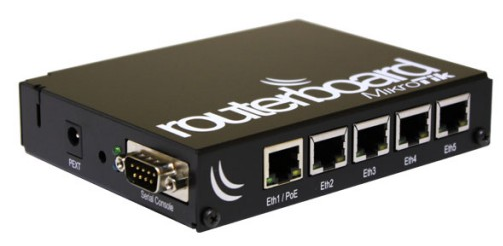
\includegraphics[scale=0.30]{images/rboard.png}
  \caption{\emph{Experience scenario}}
  \label{fig:topo}
\end{figure}

The router board that we used is MikroTik miniROUTER RouterBOARD 450G. This Router Board virtualize an OpenFlow switch that support
OpenFlow v1.0\cite{routerboard_doc}.
\begin{itemize}
   \item CPU		AR7161 680MHz
   \item Memory		256MB DDR SDRAM onboard memory
   \item Data storage	512MB onboard NAND memory chip, microSD card slot (on reverse)
   \item Ethernet 	Three 10/100/1000 Mbit/s Gigabit Ethernet ports supporting Auto-MDI/X
   \item Serial port 	One DB9 RS232C asynchronous serial port
\end{itemize}
\textbf{firmware} the current version is: '' da gercare col comando: system routerboard print ''
\newline
The \textbf{Operating System} that they use is MikroTik RouterOS ( cercare la versione installata) \cite{routeboard_software}.
\newline
One limitation of this routerboard is that it has only 5 ethernet port this is a limitation because consider that one of this port it is
used to connect conntroller and with other port we have made host and other routerboard connection.

%correggere e completare Matteo

\section{Results}\label{sec:results}
\subsection{Controller}
We developed a controller that can handle a mesh network, which has loops, that avoid
the traffic flooding. The controller stores the switch and the connection between them;
knows which hosts are connected to each switch port, with the hypothesys that only one
host is connected at each port, unless the port is the one connected to the internet.
With the use of the statistics, the controller get the status of the network and, if necessary,
tries to adjust the traffic and put in the link with the higher path loss the torrent traffic,
make the connection between two gaming host the one with less delay and tries to redistribute all the traffic in a way
such that all the nodes have an average throughput as lowest as possible.
\\
\newline
We have used some principal function released with POX controller:
\begin{itemize}
 %\item \texttt{pox.topology.launch()} and \texttt{pox.openflow.topology.launch()} descrivere a che ci serve\cite{pox}.
 \item \texttt{pox.openflow.discovery.launch()} this function run algorithm in order to discovery the network and every time in witch some new
 topological change occour it return an event with ( con cui ) we can update our topological knowledge.
 It does not provide the host event. For host event\cite{pox}.
 \item \texttt{pox.openflow.spanning_tree.launch()} this function is necessary with a presence of loop on topology
 because with a spanning_tree algorithm it avoid the broadcast storm of message. When we set up \texttt{OFPP_FLOOD} like output port action in a table's
 switch row if some spanning_tree algorithm run the \texttt{OFPP_FLOOD} is only theoretical infact the algorithm close some port for flooding service
 on the switch in orther to avoid loop\cite{pox}.
\end{itemize}
\subsection{Real Lab Scenario}
The topological scenario in which we have set up experience is the next:
\begin{figure}[!h]
 \centering
 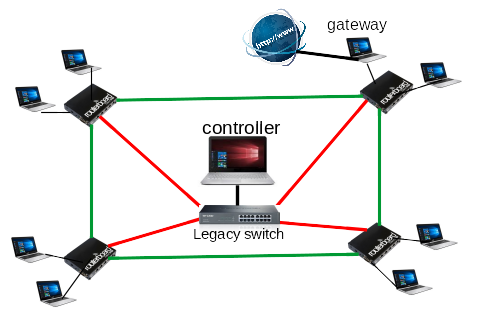
\includegraphics[scale=0.70]{images/topo.png}
 \caption{\emph{Experience scenario}}
 \label{fig:topo}
\end{figure}

We have use 4 MikroTik Router board that were provided us in the Communication Networks Lab at DEI in University of Padua.
The 4 routerboard is connected each other in order to design a loop. Every sigle board connect two host and is connected with a legacy switch that provide
to logically connected with controller.

\subsection{Graph and Network structures}
  In order to achieve the realtime adaptability and statistics storage we have develop ad-hoc structure.
  We use a specific python library called NetworkX \cite{networkx} to create a graph in witch we can storage ad-hoc node that represent
  resplectively switch or host element.
  This topological structure is updated realtime thanks to connection event and link discover offered by various library.
  ( mettere i vari eventi che sfrutto )
  The link besides have many parameters in witch we can save network performance. To update every link parameter we have to creat ad hoc function
  because there isn't some function constructed yet. ( sistemare frase) .
  This type of structure allow us to run Dijkstra algorithm that return the minimum path ( in base a vari parametri ) on a nlog n time ( verificare).
  (aggiungere qualcosa e correggere)
  
  \begin{figure}[!h]
 \centering
 \includegraphics[scale=0.30]{images/topology.png}
 \caption{\emph{Experience scenario}}
 \label{fig:topo}
  \end{figure}
  
  \#TODO matteo

  \subsection{Traffics analisis}\label{subsec:traf}
  We used laptop connected via
GigabitEthernet interface and Ethernet cable cat.5a to receive the traffic from the destination host.
Our laptop has been connected via Wi-Fi to our access point via protocol 802.11n.
No other traffic sources were active during the testing, so the router was handling only
the traffic from laptop when sniffing traffic. The connection used was an ADSL2+ via copper.
We did 3 type of traffic analysis: Gaming traffic, Skype® and torrent traffic. We analyzed
\#Mb for the gaming traffic, \#Mb for the VoIP traffic and 3GB for the torrent traffic.
The analysis involved the average number of packets per second, the packet size, the protocol (TCP or UDP)

The traffic analysis of the torrent protocol shows that the average packet size is the MTU
(i.e. 1500bytes) and the protocol tryies to exploit all the channel capabilities. The traffic
is made via UDP packets with the port range in the ephimeral ports (2000_- 65535).
Moreover, the node is linked to a lot of IPs with multiple connection: this means that
if someone wants to find a p2p traffic, it can look to the statistics and see if the traffic is loading all the channel,
to how many IPs, an host is connected to and if it uses UDP.
For the VoIP we saw that the protocol uses UDP and the traffic, after a transition time, goes only between two hosts.
The average packet size is the MTU and the protocol tryies to exploit all the channel for a better QoE.
On another test, we tried the VoIP while a download was ongoing, and we saw that the quality
decreased to allow communication. The traffic is between the UDP port 80 \#\#TODO\#\# TOCHECK \#\#

The last traffic analysis we made was with a DOTA[explain what it is] web match.
We saw that for that type of gaming session, the packet size is about \# bytes and involves both TCP and UDP ports.
  \\
  \\
  For every networks performance we have tryed to develop a specific solution. The OpenFlow main goal is to centralize controll and software
  complexity so the routerboard can made only some easy function in orther to contain the hardware complexity and mantainly a good speed\cite{qos_paper}.
  Il che ha portato a dover utilizzare stratagemmi.
  \#TODO %riformulare
    \subsubsection{Delay}
Monitoring round-trip time provides important insights for network troubleshooting and traffic engineering.
The  common  monitoring  technique  is  to  actively  send  probe packets  from  selected  vantage  points  (hosts  or  middleboxes).
In traditional  networks, the control over the network routing is
limited,  making  it  impossible  to  monitor  every  selected  path. The  emerging  concept  of  Software  Defined  Networking  sim-plifies
network  control.  However,  OpenFlow,  the  common  SDN protocol,   does   not   support   RTT   monitoring   as   part   of   its
specification. In this experience we have tryed to emply an tecnic to escape this problem\cite{rtt}.
\newline The idea is to measure the time that occure from sending a packet from controller to a switch and the time in which the packet return from
an other switch.
\\
\newline First we have to discovery round trip time from controller to every single switch on our topology.
In order to do this on the controller we start a timer, we send a proper packet to the switch specifing the \texttt{OFPP_CONTROLLER - Send to the controller}
option and when the message return to the controller we stop the timer and calculare RTT for the switch.
\begin{figure}[!h]
 \centering
 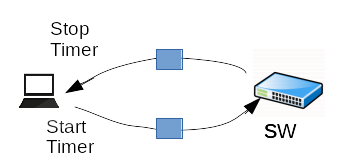
\includegraphics[scale=0.70]{images/rtt2.png}
 \caption{\emph{RTT between controller and OF switch}}
 \label{fig:topo}
\end{figure}
\newline
If we need to calculate the delay on a specific link, the rtt has to calculate with the headed switch of this link.
\\
\newline
Now we create a proper message with unique identifier number, we start a timer \texttt{TM1} and then send this message to a first switch specifing the output port.
Then when the packet comes to the second switch it identify the particular message and sends to the controller that stops it's dedicated timer \texttt{TM2}.
\newline This part required a particolar flow entry on the second switch in orther to send to the controller only some particulare packet.
\begin{figure}[!h]
 \centering
 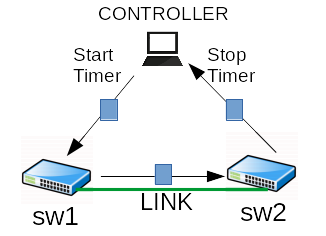
\includegraphics[scale=0.70]{images/rtt1.png}
 \caption{\emph{Pck from controller to itself following a particular way.}}
 \label{fig:topo}
\end{figure}
\\
\newline At this point we can calculate the delay of the link.
\\
\\
 delay = (TM2 - TM1) - RTT1/2 - RTT2/2
\\
\\
Teorethically this method must works but in practice there are a lot of delay introduce from computational concestion on the virtualized controller.
What we observe is a estimated delay like some seconds that is impossible, infact if we made some \texttt{ping test} from one host to another host
in this SDN network we realize delay around 3ms.
\\

		\subsubsection{Link Capacity}

	\#TODO andrea
	The first data that was collected was the actual link capacity, which depends both on the cable used to connect
	different devices and the effective capacity for each ethernet port linked by the cable itself. Everytime a device supporting
	openflow connects to the controller, it gives to the latter information about its status and its capabilities. One of them is
	the link capacity in three ways: the first is the \textit{supported} capacity, which is the phisical maximum capacity, the second is the
	\textit{advised} capacity, which name describes itself and the latter is the \textit{current} one. We choose to save the last one,
	as it gives the most useful about the link state. This information, moreover, is the one that non-SDN switches use to choose the \textit{metric}
	parameter. The simulation with Mininet showed us that this type of information can be used, but the Routeboards didn't support it.
	As a matter of fact, we weren't able to exploit this capacity in our network realization.
		\\
		\\
  \subsubsection{Throughput}
	\#TODO andrea
	Using the flow statistics, we analyzed the traffic going through a link and, with a simple division, we got the normalized throughput.
	We exploited the information given by the switches with the match structure: this means that we used the throughput for the TCP traffic,
	the one for the UDP and for each of them we could know toward which IP the traffic is directed or is from. This was exploited with mininet
	simulations, but not in the set up in the laboratory. With the latter, we used the statistics as an indicator of the bitrate of a link
	and divided the host to categories based on it.
\\
\subsubsection{Packet error rate}

The port statistics given by the switches contains different informations about the state of each port in a switch. To classify a link for its
reliability, we divided the number of packets with erroneous symbols that couldn't be corrected with a FEC by the total number of packets that were sent,
getting the packet error rate. The choice we made when exploiting this statistic was privileging the gaming and normal traffic, wherease the
heavy traffic was directed to links with highest packet error rate.  As the switches exchanges a packet before recognizing most of the error, both because the
phisical error are corrected using blocks coding and other error are found using a \textit{Frame Check Sequence} like CRC, the byte error were considered worse as
those are indirect measures themself and the error derived from the calculations could grow up.
\#TODO andrea
\\
\subsection{Route changing} %cambio rotte

\#TODO andrea
For each statistic we got and each parameter we obtained, we changed the weight of the graphs. Every graph we used had a specific weight, so the
Dijkstra algorithm for a weighted graph gave different minimum path between two hosts. From the parameter we saved, we choose to change the
route to reach the destination and viceversa. The traffic follow the same path in both the directions and depends only on the type of traffic:
we choose to set the minimum unweighted path if no statistics were available, the minimum throughput path for the standard traffic, the minimum
delay for the gaming one and the maximum packet error rate for the heavy traffic generated by a host.
Two threshold were chosen based on the traffic analysis described on Sec. \ref{subsec:traf} which are 200 bytes/s for the gaming traffic and one megabyte/s
when the node is considered in heavy traffic. Those two threshold were made as they are average values and considering that our network is made of few really fast link,
so on one side the lower limit is sufficient not to consider gaming traffic to be a normal traffic, wherease it's easy to reach the high level of traffic load between two machines.
The changing of the path were made only if the last change happened before one minute because the torrent traffic has, in its protocol, a discovery
algortithm. This means that if a lot of changes were made, most of the traffic generated by the peer to peer, is the control one and the result is that the
load in the network will be heavy and last longer.

\subsection{ARP solution}

During our analysis and in our tests, we prove that in a SDN mesh network, the ARP packets are useless.
This type of packets is useful for a multipoint to multipoint connection where the connection is set between a
HUB and a set of computers or between a bridge and a computer. The first case is no more in use in common networks as
it higher the collision range. The bridges limits their collision range to the port. With openflow each switching unit can
act as a bridge or as a router. In both cases analyses the header of the L2 packet L3 packet and some of the L4 header.
If it has the rule to forward the packet, it will act as declared in the most specific matching rule. Otherwise it will
send to the controller a PacketIn and the controller will act as programmed. If an host want to communicate to another host whithin
the network, it sends the packet to the line and then the switch will check in its tables and execute the actions of the match found.
For an IP network, it will check the path to reach a destination and then send to the defined output port. The mac address in this case
became useless, as the connection is point to point. So, knowing the destination layer2 address is useless as the switch can act
regardless of it. The only thing the switch need to know is the layer2, layer 3 addresses and, at most, the layer 4 address.
This can be seen by a reader as a violation of the layers in the ISO/OSI stack, but to exploit the potentials of the SDN approach,
this is necessary.

\subsection{Default Gateway}
Analyzing the traffic while we were trying the controller on real machines in the lab, we have tried to set the default gateway to
other machines that were connected to the SDN network, but not to the internet. We proved that the controller can redirect correctly the
traffic to the internet. This means that
computers don't need anymore to set a gateway to reach another network as the controller and the switches will redirect the traffic
properly, according to the rules set by the first. The controller must only know which switch ports are connected to the
internet and then add them to the path. I this way, the controller can set a path to reach it and provide connectivity with
a traffic shaping policy and/or differentiate the traffic from and to different networks.

\subsection{Ip switching in pox}

During our tests, both with Mininet and in the lab, we found out that the core of POX, when a PacketIn event occoures, switches the source and the destination addresses,
both MAC and IP, if one of the hosts is already known. We weren't able to understand in which point of the code of POX  and why it happens.
% One of the problem encountered was that, if an host is already found by pox and there is a PacketIn event, the core of the controller
% switches the source and the destination IP and MAC address with the source one.
The problem was partially solved, checking out the
parameters known by the controller, i.e. if the two host are connected to two different switches and the controller switches the source with the
destination address, we can switch it back; the result is that the PacketIn event now has correct informations.
If the two host are in the same switch, the problem is solved using a controlled packet flooding, described in section \ref{sec:connectivity}

\section{Conclusions}\label{sec:conclusion}
Conclusions are a superbrief summary of what has been done and highlighting of the "take home message"
ehi
\#TODO


\begin{thebibliography}{99}
	\bibitem{pox} POX \url{https://openflow.stanford.edu/display/ONL/POX+Wiki}
	\bibitem{openflow} OpenFlow \url{http://flowgrammable.org/sdn/openflow/}
	\bibitem{pox_repo} POX's repository \url{https://github.com/noxrepo/pox}
	\bibitem{VM} Virtual Machine \url{http://sdnhub.org/tutorials/pox/}
	\bibitem{router_board} Router Board \url{https://www.senetic.it/product/RB450G}
	\bibitem{networkx} NetworkX python's library \url{https://networkx.github.io/}
	\bibitem{ONF} Open Networking Foundation \url{https://www.opennetworking.org/sdn-resources/technical-library}
	\bibitem{ONF_report} v1.5.1 OpenFlow report \url{https://www.opennetworking.org/sdn-resources/technical-library}
	\bibitem{routerboard_doc} RouterBOARD 450G MikroTik documentation \url{http://www.routerboard.sk/files/pdf/rb450g_manual.pdf}
	\bibitem{routeboard_software} RouterBOARD MikroTik Software \url{https://mikrotik.com/software}
	\bibitem{farzaneh}  Efficient Topology Discovery in Software Defined Networks F. Pakzad, M. Portmann, W. L. Tan and J. Indulska
	School of ITEE, The University of Queensland Brisbane, Australia \url{https://www.researchgate.net/publication/271508903_Efficient_Topology_Discovery_in_OpenFlow-based_Software_Defined_Networks}
	\bibitem{qos_paper} OpenNetMon: Network Monitoring in OpenFlow Software-Defined Networks Niels L.
	M. van Adrichem, Christian Doerr and Fernando A. Kuipers Network Architectures and Services, Delft University of Technology
	Mekelweg 4, 2628 CD Delft, The Netherlands \url{https://pdfs.semanticscholar.org/ea94/7a9334484ee4c3bb6bcfb4d1590aece1b178.pdf}
	\bibitem{rtt} Efficient Round-Trip Time Monitoring in OpenFlow Networks A. Atary A. Bremler-Barr Interdisciplinary Center Herzliya \url{http://www.deepness-lab.org/pubs/infocom2016_grami.pdf}


	\end{thebibliography}

\end{document}
